\documentclass{beamer}
\usetheme{CMU}

\usepackage{pgf,pgfarrows,pgfnodes,pgfautomata,pgfheaps,pgfshade}
\usepackage{amsmath,amssymb}
\usepackage[utf8]{inputenc}
\usepackage{colortbl}
\usepackage[english]{babel}
\usepackage{booktabs}
\usepackage{slpython}
\usepackage{underscore}

\author{Luís Pedro Coelho}
\institute{Programming for Scientists}

\graphicspath{{figures/}{figures/generated/}{images/}}

\newcommand*{\code}[1]{\textsl{#1}}


\makeatletter
\def\verbatim@font{\small\ttfamily}
\makeatother
\title{Software Carpentry I: The Shell \& Version Control}
\begin{document}
\frame{\maketitle}

\begin{frame}[fragile]
\frametitle{Software Carpentry}

\alert{Software engineering} helps you build the equivalent of a bridge.

\medskip

\alert{Software carpentry} is what you need to build the equivalent of a garden shed.

\note{
    Coined by Greg Wilson, U. of Toronto.

    Not part of the original plan for the class, but then I found the software carpentry website.
}

\end{frame}

\begin{frame}[fragile]
\frametitle{Basic Tool: Shell}
\note{
If you remember using MS-DOS, then that's crap. Interestingly, MS now makes one very interesting shell (PowerShell).

Don't be afraid of the shell.
}

\centering
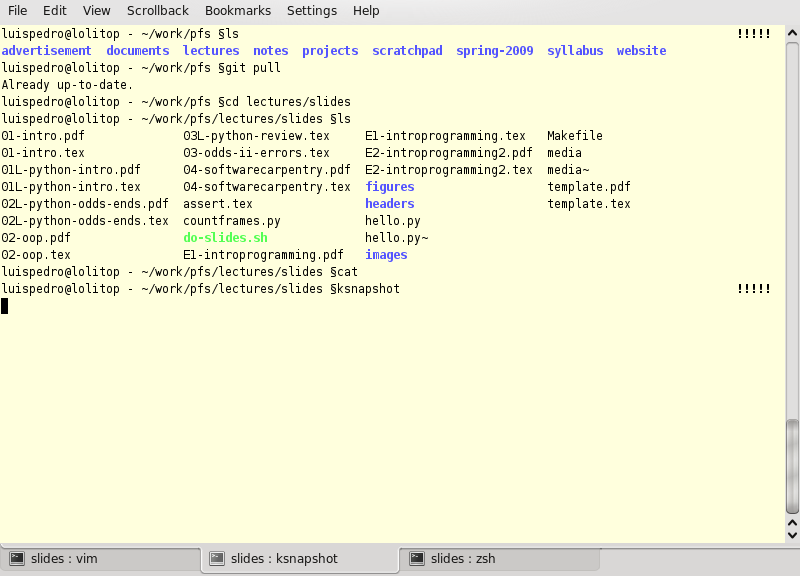
\includegraphics[width=.9\textwidth]{04-konsole.png}

\end{frame}

\begin{frame}[fragile]
\frametitle{Basic Concepts}

\begin{itemize}
\item Current directory.
\end{itemize}

\texttt{cd newdir}

\end{frame}

\begin{frame}[fragile]
\frametitle{Directories}

Your program also has a current directory.

\begin{python}
import os
os.chdir('..')
\end{python}

\end{frame}

\begin{frame}[fragile]
\frametitle{Paths}
\begin{itemize}
\item \alert{Absolute paths:} \texttt{/home/luispedro/work/pfs/lectures/slides/04-softwarecarpentry.pdf}
\item \alert{Relative paths:} \texttt{04-softwarecarpentry.pdf}, \texttt{../homeworks/02-oop.pdf}
\end{itemize}
\end{frame}

\begin{frame}[fragile]
\frametitle{Executing Programs}

\begin{verbatim}
luispedro@lolitop - ~/work/pfs/lectures §
\end{verbatim}

\end{frame}

\begin{frame}[fragile]
\frametitle{Executing Programs}

\begin{verbatim}
luispedro@lolitop - ~/work/pfs/lectures §ls
01-intro-python.pdf  02-oop.pdf  03-python-odds.pdf
do-hw.sh  Makefile 01-intro-python.tex  02-oop.tex
03-python-odds.tex  headers
luispedro@lolitop - ~/work/pfs/lectures §cat Makefile
pdfs := $(patsubst %.tex,%.pdf,$(wildcard *.tex))
all: $(pdfs)

.PHONY: all

%.pdf: %.tex
        ./do-hw.sh $<
luispedro@lolitop - ~/work/pfs/lectures §vim 03-python-odds.tex
luispedro@lolitop - ~/work/pfs/lectures §
\end{verbatim}

\end{frame}

\begin{frame}[fragile]
\frametitle{Input/Output}
\begin{block}{hello.py}
\begin{python}
print 'Hello World'
\end{python}
\end{block}

\begin{block}{Shell}
\texttt{python hello.py}
\end{block}
\end{frame}


\begin{frame}[fragile]
\frametitle{Input/Output}
Standard input/stdout.
\end{frame}

\begin{frame}[fragile]
\frametitle{grep}

\begin{verbatim}
lp@lolitop ~/pfs/lects/slides §grep Exception *tex
01-intro.tex:\item Exception: implementing code from a paper.
03-odds-ii-errors.tex:\frametitle{Exceptions}
03-odds-ii-errors.tex:\begin{block}{Exceptions}
03-odds-ii-errors.tex:\frametitle{Exceptions}
03-odds-ii-errors.tex:\frametitle{Exceptions}
03-odds-ii-errors.tex:\begin{block}{Exceptions}
03-odds-ii-errors.tex:\item Exceptions are \alert{objects}.
03-odds-ii-errors.tex:\item Exceptions have \alert{type} and \alert{values}.
03-odds-ii-errors.tex:\frametitle{Exception Hierarchy}
03-odds-ii-errors.tex:               Exception
03-odds-ii-errors.tex:\frametitle{Exception Handling}
03-odds-ii-errors.tex:\begin{block}{Exception Handling: Error Handling}
03-odds-ii-errors.tex:    print 'Exception'
03-odds-ii-errors.tex:False\\Exception
03-odds-ii-errors.tex:True\\Exception
04-softwarecarpentry.tex:grep Exception *tex
\end{verbatim}

\end{frame}

\begin{frame}[fragile]
\frametitle{wc}
\begin{block}{WC: Word Count}
\texttt{wc -l}: count lines
\end{block}
\end{frame}

\begin{frame}[fragile]
\begin{verbatim}
lp@lolitop ~/pfs/lects/slides §grep Exception *tex | wc -l
19
\end{verbatim}
\end{frame}

\begin{frame}[fragile]
\frametitle{Command-line Arguments}
\begin{verbatim}
grep Exception *tex
\end{verbatim}
\end{frame}

\begin{frame}[fragile]
\frametitle{Levels}
\begin{enumerate}
\item konsole/xterm/gnome-terminal/iTerm.app/Terminal.app/\ldots
\item sh/bash/zsh/\ldots
\item your program
\end{enumerate}
\end{frame}

\begin{frame}[fragile]
\frametitle{Command-line Arguments}

\begin{verbatim}
luispedro@lolitop - ~ §echo Hello World
Hello World
\end{verbatim}
\end{frame}

\begin{frame}[fragile]
\frametitle{Command-line Arguments}

\begin{python}
import sys
print len(sys.argv)
print sys.argv
\end{python}
\end{frame}

\begin{frame}[fragile]
\frametitle{Command-line Arguments}

\begin{verbatim}
§python printargs.py Hello World
3
['printargs.py', 'Hello', 'World']
\end{verbatim}
\end{frame}

\begin{frame}[fragile]
\frametitle{Command-line Arguments}

\begin{verbatim}
§python printargs.py "Hello World"
2
['printargs.py', 'Hello World']
\end{verbatim}
\end{frame}

\begin{frame}[fragile]
\frametitle{Command-line Argument Parsing}

\begin{python}
from optparse import OptionParser                        
parser = OptionParser()                                  
parser.add_option("-d", "--database", dest="database")   
parser.add_option("-i", "--ideal-scale", dest="ideal")   
parser.add_option("-m", "--min-scale", dest="min")       
parser.add_option("-M", "--max-scale", dest="max")       
(options, args) = parser.parse_args()                    

Elsevier_DB=options.database
Ideal_Scale=float(options.ideal)
Min_Scale=float(options.min)
Max_Scale=float(options.max)
\end{python}
\end{frame}

\begin{frame}[fragile]
\frametitle{Commands}

\begin{itemize}
\item cd
\item ls
\item cat
\item grep
\item \ldots
\end{itemize}
\end{frame}

\begin{frame}[fragile]
\frametitle{SSH}
\begin{block}{Secure Shell}
\begin{verbatim}
§ssh coupland.cbi.cmu.edu
\end{verbatim}
\end{block}
\end{frame}

\begin{frame}[fragile]
\frametitle{Password-less Login}
Public key authentication.
\end{frame}

\begin{frame}[fragile]
\frametitle{Version Control}

If your laptop exploded, how many hours of work would you lose?
\end{frame}

\begin{frame}[fragile]
\frametitle{Advantages}
\begin{itemize}
\item Maintain project history.
\item Sync between computers.
\item Sync between project members.
\item \ldots
\end{itemize}
\end{frame}

\begin{frame}[fragile]
\frametitle{Subversion}
\begin{block}{Subversion: model}
\begin{enumerate}
\item Repository
\item Checkout
\item Commit
\end{enumerate}
\end{block}
\end{frame}

\begin{frame}[fragile]
\frametitle{Example}
\begin{enumerate}
\item Create a repository
\item Create a checkout
\item Edit
\item Commit
\end{enumerate}
\end{frame}

\begin{frame}[fragile]
\frametitle{Version Control Etiquette}
\begin{itemize}
\item Don't commit over my commit.
\item Use the log.
\end{itemize}
\end{frame}

\end{document}
